%!TEX root = ../template.tex
%%%%%%%%%%%%%%%%%%%%%%%%%%%%%%%%%%%%%%%%%%%%%%%%%%%%%%%%%%%%%%%%%%%%
%% chapter4.tex
%% NOVA thesis document file
%%
%% Chapter with lots of dummy text
%%%%%%%%%%%%%%%%%%%%%%%%%%%%%%%%%%%%%%%%%%%%%%%%%%%%%%%%%%%%%%%%%%%%

\typeout{NT FILE chapter4.tex}%
\chapter{System Design}
\label{cha:system_design}
This chapter presents the overall design and conceptualization of the system developed. It begins in Section \ref{sec:requirements} with a description of the system requirements, followed by Section \ref{sec:tools} that introduces the technologies and tools adopted.
Subsequently, an overview of the system architecture is analysed in Section \ref{sec:architecture} and the database structure is presented in Section \ref{sec:database}.
Finally, it ends with a discussion of the implementation choices made, in Section \ref{sec:discussion_design}.

\section{Requirements}
\label{sec:requirements}

This section describes the requirements of this dissertation, categorized into the following areas: Interactive Map, \gls{3D} Model Interaction, and Virtual Reality (\gls{VR}) environment.

\subsection*{Interactive Map}
A map of the Troia archaeological site to offer interactive functionalities.
\begin{itemize}
    \item \textbf{Map Navigation:} Users can navigate in the environment, and explore different locations.
    \item \textbf{Perspective Switching:} Toggle between top-down and profile views for better spatial understanding.
    \item \textbf{Layer Toggle:} Toggle visibility of layers, overlay a \textit{.tif} map illustration, such as excavation campaigns.
\end{itemize}

\subsection*{\gls{3D} Models \& Interaction}
A focus on the interaction with \gls{3D} models, which are integrated into a \gls{VR} environment.
\begin{itemize}
    \item \textbf{Artifact Interaction:} Allows users to virtually manipulate the glass artefact models.
    \item \textbf{Contextual Overlay:} Display descriptive data about the artefact, such as its origin, period, and historical usage.
    \item \textbf{Reconstructed Models:} Showcase how artefacts would look originally (having in consideration characteristics such as: colourless glass, archaeological drawings and symmetry). 
    \item \textbf{3D Models Integration:} The user can zoom the map to visualize the perspective of a specific \gls{3D} model.
    %select a position to visualize the perspective of their 3D model.
\end{itemize}

\subsection*{\gls{VR} Environment}
\gls{VR} functionalities to provide an intuitive \gls{UX}, enabling interaction with the \gls{VE} through the use of \glspl{HMD}.
\begin{itemize}
    \item \textbf{Immersive Experience:} \gls{VR} allows users to immerse in a virtual tomb visit, enabling interaction with glass relics.
    \item \textbf{Device Accessibility:} Primarily user-friendly and enabling haptic interaction, while supporting \gls{VR} glasses as an emerging display option.
    \item \textbf{Localization \& Wayfinding:} 
    \begin{itemize}
        \item \textbf{\gls{POI}:} Use colors, text, visual markers, or direction arrows to emphasize and guide users to historically significant locations.
    \end{itemize}
   % \item \textbf{Multilingual Support:} Provide language options to ensure accessibility for an international audience.
\end{itemize}

\section{Adopted Tools and Tecnhologies}
\label{sec:tools}
The following section focuses on the technologies and tools used in implementing this project. 
These include environments used, Unity engine, development tools, backend, and data management.
\subsection{Working Environment}

The  \gls{VR} environment was developed using the Unity editor, with code scripts written in C\# within the \textbf{Visual Studio Integrated Development Environment (IDE)}\footnote{\url{https://visualstudio.microsoft.com/}}.
Its features, such as debugging tools, error detection, code navigation, Unity-specific types recognized automatically, and IntelliSense suggestions, greatly enhanced productivity. 
To further support this integration, the Visual Studio Editor package was used. 

For the backend implementation, comprising the Node.js server and the database, \textbf{Visual Studio Code (VSCode)}\footnote{\url{https://code.visualstudio.com/}} was used. 

The version control system used initially for project management was \textbf{GitHub}\footnote{\url{https://github.com/}}, providing effective tracking of updates and overall code organization.
However, as a consequence of storage limitations in handling large files, such as the \gls{2D} ground view or the funerary enclosure \gls{3D} model, the \textbf{Diversion}\footnote{\url{https://www.diversion.dev/}} tool was employed as an alternative solution for managing these system.

\subsection{Unity}
\textbf{Unity} is a cross-platform engine that provides a robust environment for developing \gls{2D} and \gls{3D} applications. 
Its component-based architecture simplifies \gls{3D} development by allowing developers to define object behaviors through scripts in Virtual Environments (\glspl{VE}).
Unity also offers a community forum and repositories available in \textbf{Unity Asset Store}\footnote{\url{https://assetstore.unity.com/}} where developers can access resources and adapt them for their projects.

For this study, Unity was selected for developing the \gls{VR} environment. The C\# programming language used within Unity facilitates the management of game objects and user interactions in the \gls{VE}.
Its integration enables users to have an immersive experience while interacting with the \gls{UI}, using the \gls{HMD}.
The headset device used for testing during the implementation and for user evaluation was \textbf{Meta Quest 3}.

\subsubsection{Unity Packages and Plugins}
This section comprises the main assets, plugins, and components used to support the custom implementation.

The following packages of Unity Asset Store were used to enhance the \gls{UI} and streamline the development process:

\begin{itemize}
\item{\textbf{Free UI Click Sound Pack}\footnote{\url{https://assetstore.unity.com/packages/audio/sound-fx/free-ui-click-sound-pack-244644}} - This package provides a collection of diverse clickable sounds, designed to provide an immersive and complete \gls{UX}.}
\item{\textbf{Simple Pie Menu}\footnote{\url{https://assetstore.unity.com/packages/tools/gui/simple-pie-menu-radial-menu-asset-270056}}} - A radial menu system implemented as the main menu of the project. Further details on its functionality are provided in Section \ref{sec:main_menu}.
\item{\textbf{White \& Black GUI}\footnote{\url{https://assetstore.unity.com/packages/2d/gui/icons/white-black-gui-by-gamertose-168805}}} - This package includes a range of trivial and useful icons used to guide users in navigating menu items and to support image gallery switching between pre- and post-intervention object states.
\end{itemize}



The \textbf{XR Plugin Management} package was used to simplify the integration and management of various XR plug-ins. 
This package is primarily responsible for loading, initializing, configuring settings, and providing build support for XR features. 
It was used in conjunction with the OpenXR. \textbf{OpenXR} is an open-standard \gls{API} enabling cross-platform development, with a high-performance access to \gls{AR} and \gls{VR} platforms and devices. In this study, this plugin handles communication with the \gls{VR} headset.

Diverse components of the \textbf{XR Interaction Toolkit}\footnote{\url{https://docs.unity3d.com/Packages/com.unity.xr.interaction.toolkit@3.0/manual/components.html}} were integrated and added to the Unity Inspector, abstracting much of the low-level complexity of \gls{VR} development. It enabled features such 
as Object interaction (grab and release), Teleportation-based locomotion, \gls{UI} interaction, and Controller support.
For interaction within the virtual scene, the \textbf{XR Near-far interactor} was added and provided a way to interact with the scene through the ray emitted from the controllers, and the \textbf{XR Grab Interactable} enabled direct manipulation of virtual objects through grabbing, holding, and releasing actions.

Its \textbf{XR Origin} structural component served as the root GameObject that encapsulated the main camera and controller setup. 
It handled camera tracking based on the user's head movement and managed controller positioning and orientation. 
Furthermore, to implement user movement within the \gls{VE}, a Locomotion System was added with the following components integrated: 

\begin{itemize}
\item{\textbf{Continuous Move Provider:}  Allowed smooth movement via the right joystick.}
\item{\textbf{Snap Turn Provider:}  Enabled rotational movement in fixed increments, chosen over continuous turning to reduce motion sickness.}
\item{\textbf{Teleportation Provider:} Enabled teleportation across the plane surface using the left joystick.}
\item{\textbf{Teleportation Anchors:} Defined specific teleportation points, represented as buttons.}
\end{itemize}

For input handling, this toolkit provides two systems: the old Input Manager and the newer \textbf{Input System Package}. 
While the \textbf{Input Manager} is built into the Unity engine and used by default, the project adopted the Input System Package due to its flexibility and scalability. 
This newer system supports a wide range of input devices and enables precise configuration through a centralized interface. Input actions are defined and managed using the Input Action Manager, which allows the developer to specify actions and map them to devices or controls. 
Each input action is activated as needed during runtime, offering adaptable input handling.



\subsection{Tools}
\textbf{Blender}\footnote{\url{https://www.blender.org/}} is an open-source computer graphics software useful to a wide range of tasks, such as model, animate, create textures, materials. 
This tool was used to create an aproximation of the original texture of the glass object. Originally transparent, translucent.

\textbf{GIMP}\footnote{\url{https://www.gimp.org/}}, an open-source cross-platform image editor, was used to edit the map draw for integration as ground in Unity (rotated and cropped).
Additionally, GIMP was useful in editing the post-intervention object images. The object's images were cut out from their backgrounds, which were then replaced with a neutral grey. 
This enhanced clarity for users and allowed easy comparison between the object's before and after the cleaning and conservation treatment.

\subsubsection{Photogrammetry}
\label{sec:photogrammetry_tool} 

The software used to process digital images and generate the \gls{3D} model of the funerary enclosure was \textit{Agisoft Metashape}\footnote{\url{https://www.agisoft.com/}}.
This software performs photogrammetric processing of digital images to generate \gls{3D} spatial data, which can be applied in various fields such as \gls{GIS} applications, \gls{CH} documentation, visual effects production, and indirect measurements of objects of diverse scales. 

 A total of 143 images were collected after the excavation campaign by the archaeologist responsible for this site, Inês Vaz Pinto.
 % by the restoration department of NOVA for analysis. 
Based on these images, a \gls{3D} model of the funerary enclosure was generated, as described in Section \ref{sec:build_model}.
As part of the collaboration with the institutions, two already built models of artefacts, were provided by Sofia Pires.

\subsection{Backend \& Data Management}
This section includes the backend and database repository technologies choices. 
\subsubsection{Backend}

The backend technology selected for this thesis was \textbf{Node.js}, an open-source, cross-platform JavaScript runtime environment. 
Node.js enables developers to create servers, web applications, command-line tools, and automation programs.

In this thesis, Node.js was used to support the web server and to improve performance and scalability when handling repository data. 
Additionally, it mediates the communication between Unity and the database repository.

Express.js\footnote{\url{https://expressjs.com/}} is the most popular Node.js web application framework, widely used for building web applications and \glspl{API}, with a minimal and flexible design.
In this study, the web server Express.js was used to expose the \gls{REST}\footnote{\url{https://www.ibm.com/think/topics/rest-apis}} endpoints.


\subsubsection{Database Repository}
\label{sec:repos}

There are several alternatives for storage management systems, but the option shelt for this project was \textbf{PostgreSQL} for its geographical extension, PostGIS, and its relational database is more appropriate due to its flexibility and consistency.
Additionally, because of its high performance and flexibility in managing spatial data. 

PostGIS is widely used for spatial data storage, geometry processing, and efficient geospatial data querying.


\section{System Architecture}
\label{sec:architecture}

The system is divided into three application layers.
The \textbf{Presentation Layer} manages the \gls{VR} environment and its interaction with users. The \textbf{Application Layer} includes the management of Unity Requests, with the support of the framework "UnityWebRequest"\footnote{\url{https://docs.unity3d.com/6000.2/Documentation/ScriptReference/Networking.UnityWebRequest.html}}, acting as an intermediate between the Unity client and the database. 
The communication flow between these layers is managed through a Node.js \gls{REST} \gls{API}, chosen for its flexibility and lightweight design. 
Finally, the \textbf{Data Access Layer} contains the database, which stores all information related to object data, excavation, and object interventions. 
The architecture of the system can be observed in Figure \ref{fig:architecture}.
\begin{figure}[h!]
    \centering
    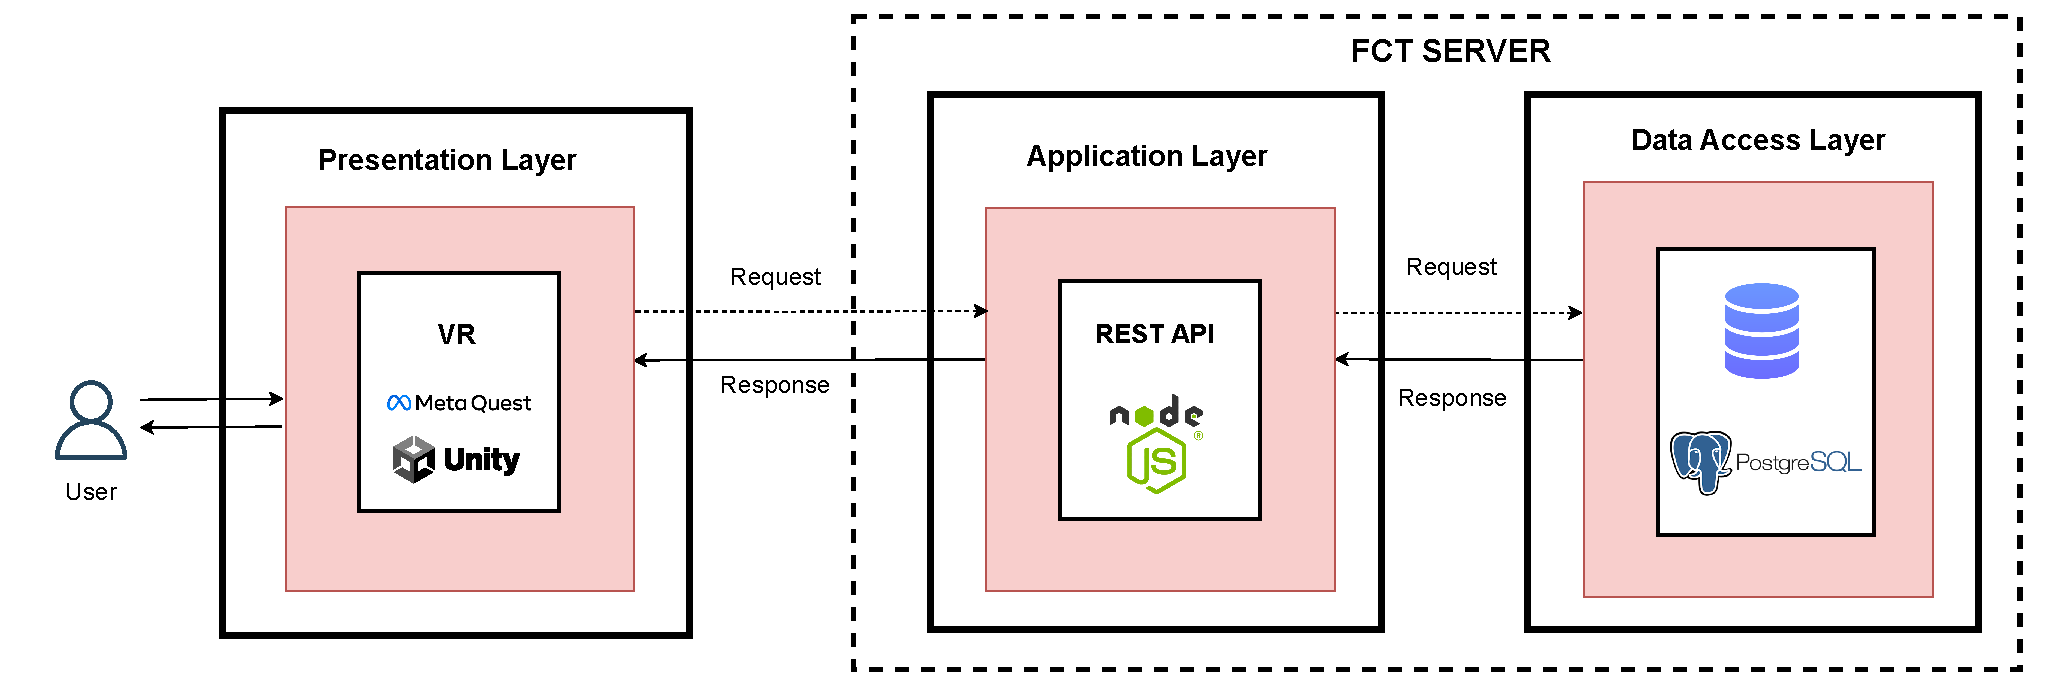
\includegraphics[width=1\linewidth]{Diagrama_Arquitetura}
    \caption{System Architecture Overview of the Developed System. \textcopyright\ Ana Maissa Antunes}
    \label{fig:architecture}
\end{figure}

During the development stage, the database was hosted locally on a PostgreSQL server managed via pgAdmin\footnote{\url{https://www.pgadmin.org/}}, an open source management tool for PostgreSQL. To access and present data in Unity, it was necessary to manually execute the "index.js" file, which contained the Node.js API endpoints.
Subsequently, before the user testing phase, the code, comprising both the \gls{API} endpoints and the PostgreSQL database, was deployed to the \gls{FCT} Server with a dedicated service.
This deployment ensured that the server hosting the \gls{API} endpoints remained continuously active, allowing Unity clients to retrieve data seamlessly without manual intervention.


\section{Database Structure}
\label{sec:database}

The database consists of 11 tables that ensure the significant data of excavation and objects are stored. %All artefacts data, excavation details, and objects intervention data were stored within this repository.
The database model was designed considering future extensibility. Initially, it was structured to store significant data from the necropolis, including the funerary enclosure and tomb under study. The structure was generalized to improve scalability, flexibility to possibly include data, such as other tombs, associated objects, and aggregate the maximum information. 
Throughout the thesis period, the database structure was continuously refined and restructured with new tables, relations, and data fields.

It was decided not to store the entire object images as binary data in the database. Instead, only file paths to the images were saved. This allowed for efficient access and manipulation of images, while other object-related data, such as text and links, was fully stored in the database.

The entities of the database, along with their main attributes and relationships, are described below, representing the necropolis, funerary enclosures, tombs, objects, and excavation data.
The \texttt{necropolis} table is the top-level table and contains general information about the site.  
The funerary enclosure or mausoleum is represented by the table \texttt{mausoleum}, which stores information such as \emph{dimensions} and \emph{construction\_materials} and references the corresponding \emph{id} in \texttt{necropolis}. The tomb within the mausoleum is represented by the table \texttt{tomb} and has a foreign key \emph{id} referencing the associated mausoleum.  
While the \texttt{tomb\_belonger} links tombs via its \emph{id}. The table \texttt{object} stores all information of each object, with 27 attributes describing each artefact. 
Moreover, table \texttt{object\_intervention} stores data about interventions performed by \gls{VICARTE}, including \emph{images\_path\_b\_interv} and \emph{images\_path\_a\_interv}, representing images of the object before and after the intervention. This table references the \emph{id} in the table \texttt{object}. Each object also has an associated table \texttt{location}, encompassing the coordinates of each object.  
Finally, the \texttt{excavation} contains excavation information, with two child tables: \texttt{excavation\_protection} and \texttt{excavation\_area}, inheriting the \emph{id} of \texttt{excavation}.  

In Unity, only the following attributes are retrieved and presented in the \gls{VR} environment: from \texttt{object}, \emph{id}, \emph{name}, \emph{material}, \emph{provenance}, and \emph{dimensions}; from \texttt{object\_intervention}, \emph{images\_path\_b\_interv}, and \emph{images\_path\_a\_interv}.

The detailed structure, including relationships and attributes, is illustrated in Figure \ref{fig:database}.

\begin{figure}[h!]
    \centering
    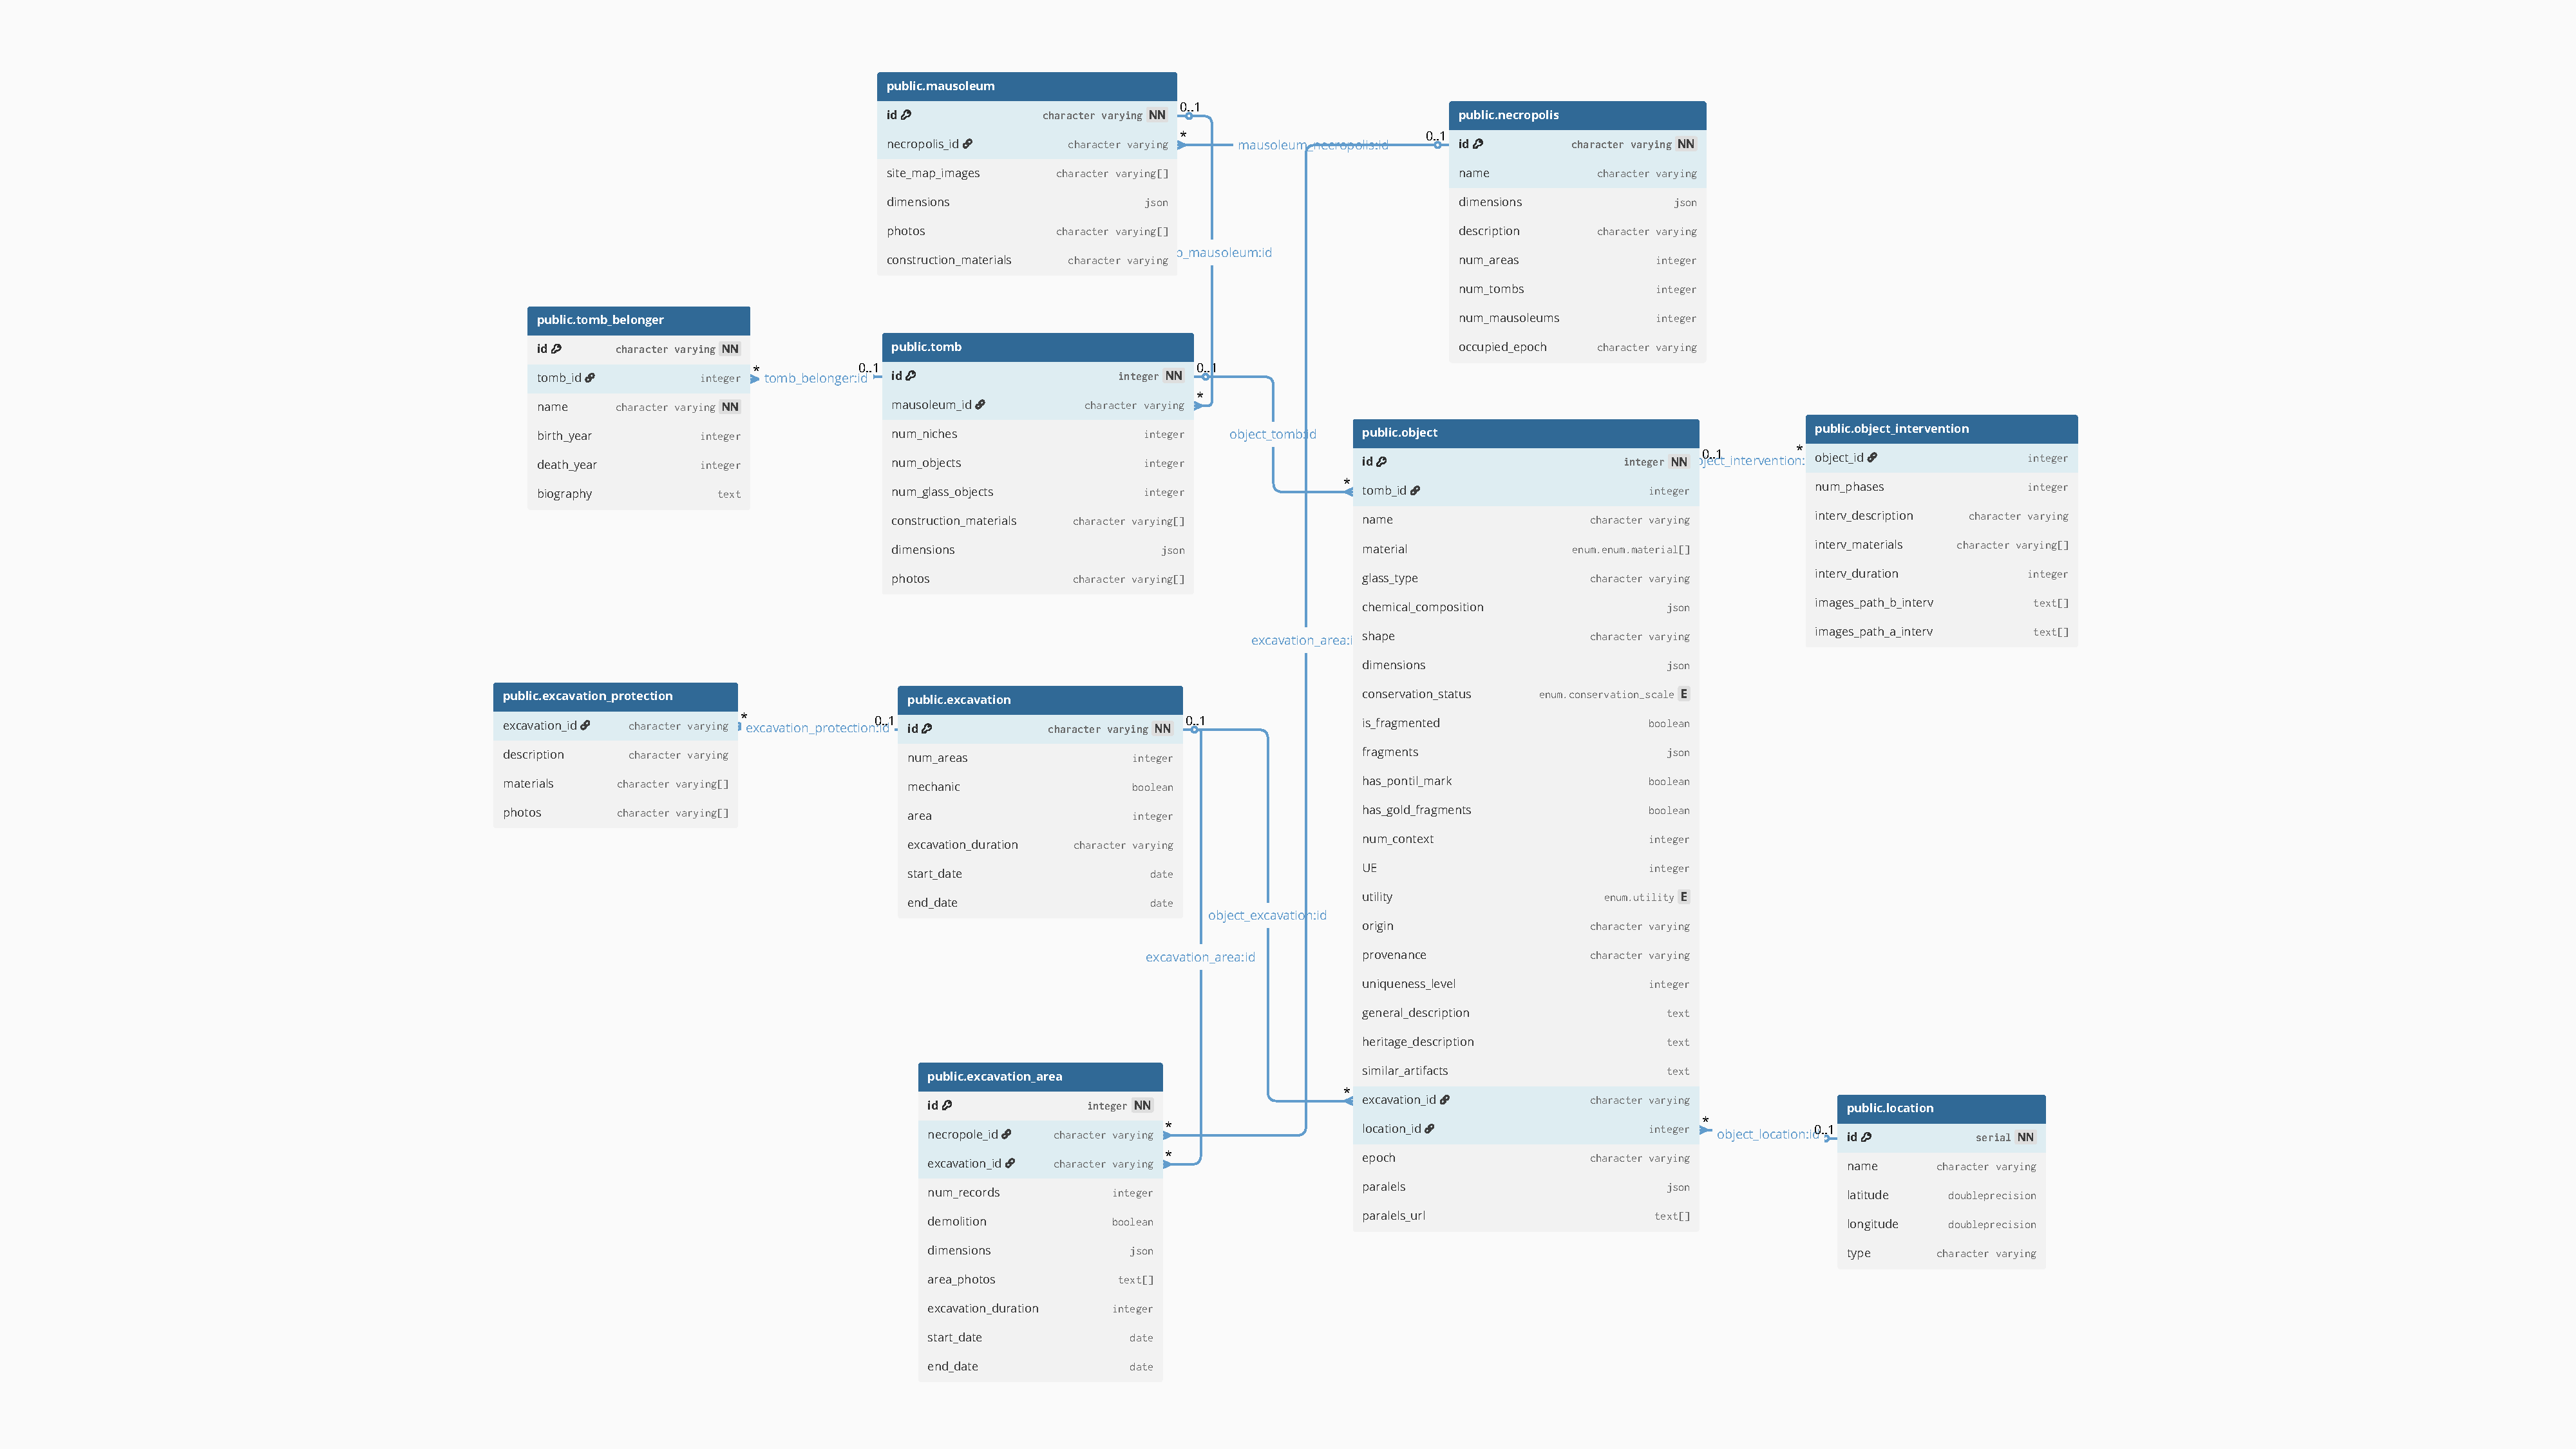
\includegraphics[width=1\linewidth, trim=13cm 0cm 13cm 0cm, clip]{thesis_db_}
    \caption{Relational Database Model.} 
    \label{fig:database}
\end{figure}


For generating the data model, SQL was used to create a database dump.
Using "dbdiagram.io", this dump was translated into a visual diagram showing tables and their relations. This tool streamlined the creation of the Entity-Relationship diagram through code.

\FloatBarrier
\section{Discussion} %resumo do capitulo + opcoes tomadas
\label{sec:discussion_design}

Given the diverse requirements of this project, the primary focus was on developing an immersive \gls{VE}, prioritizing \gls{3D} models and \gls{VR} functionalities for exploring glass artefacts within the tomb. Although interactive map features were included, they were implemented with a lower level of detail.
At the beginning of the dissertation, the development of the \gls{VR} environment and the database proceeded in parallel. Once the base database structure was implemented, the main focus was on the construction of the \gls{VE}. The initial idea was to implement the map using JavaScript and the Leaflet.js\footnote{\url{https://leafletjs.com/}} library. However, the dissertation's direction shifted towards integrating the map with the funerary enclosure and its elements directly in Unity, forming a unified \gls{VE}. This allowed users to walk across the map as if in reality, while simultaneously visualizing the \gls{3D} models accurately positioned in space.







